\documentclass[a4paper,12pt,french]{book}
\usepackage[margin=2cm]{geometry}
\usepackage[thinfonts]{uglix2}
\nouveaustyle
\begin{document}
\section*{Organisation du CCF d'algorithmique en SIO1}
\subsection*{Extrait du référentiel officiel}

Le document original est disponible \link{https://www.reseaucerta.org/sites/default/files/sio/BTS_ServicesInformatiquesOrganisations2019.pdf}{à cette adresse}.\\


Cette évaluation est constituée d'un oral de 20 minutes précédé d'une heure de préparation. Le
candidat présente sa solution algorithmique et son implémentation (durée 10 minutes maximum),
puis participe à un entretien d'explicitation conduit par la commission (durée 10 minutes maximum).
La préparation se déroule en deux parties :
\begin{enumerate}[--]
	\item une première partie de 30 mn, sur table, qui fait l'objet d'une trace écrite susceptible d'être
    examinée par la commission ;
    \item une seconde partie de 30 mn sur un équipement dédié mis à disposition par le centre
    d'examen. Durant cette phase, le candidat peut librement accéder à l'aide syntaxique
    éventuellement disponible dans l'environnement de mise en œuvre du langage utilisé.
    \end{enumerate}
La commission d'interrogation est constituée du professeur chargé de l'enseignement du module.

\subsection*{Proposition d'organisation nationale}

Le document original est disponible \link{https://siec.education.fr/fileadmin/candidats/Candidats_BTS/BTS_SIO/annexes_5_a_5-4_epreuve_E2-U22_Algorithmique_appliquee_-_SIO_2019.pdf}{à cette adresse}.\\

%\includegraphics[width=17cm]{img/planning}

\subsection*{Besoins matériels et humains}

Pour organiser l'examen comme ci-dessus, il faudrait qu'un\cdot e assistant\cdot e d'éducation surveille les deux candidats qui prépareront l'épreuve.\\
Il n'y a aucun inconvénient à ce que les candidats partagent la même salle. L'interrogation orale devrait s'effectuer dans une salle à proximité de la première, préférablement munie d'un rétroprojecteur.
Il faudrait que les trois machines soient équipées du logiciel Python pour que les candidats puissent implémenter et présenter leurs solutions.
Vu le nombre d'élèves (32 à l'heure actuelle), 3 journées devraient y être consacrées.

\subsection*{\'Eléments de réponses aux besoins}

Je pourrais rencontrer le\cdot a ou les assistant\cdot e\cdot s d'éducation pour leur expliquer brièvement le déroulement de l'épreuve. Il serait possible de les faire commencer à 9: 00 puisque je pourrai surveiller les préparations de 8: 00 à 9: 00. De même, ils pourraient terminer à 16 : 50.\\
En définitive leur présence serait requise 
\begin{enumerate}[--]
	\item de 9: 00 à 11: 40 (de 10: 00 à 11: 40 pour la 3\eme journée).;
    \item de 13: 10 à 16: 50 \\
\end{enumerate}

En ce qui concerne les salles, nous pourrions sans doute faire préparer les candidats en salle C202 Perm, traditionnellement dédiée à l'étude. Puisque celle-ci est calme peut-être que les autres élèves voulant profiter de la salle comme à leur habitude (il y en a très peu si je ne m'abuse) pourraient le faire.\\
Je me chargerais de demander à notre \textsc{AMI} d'installer les logiciels nécessaires sur les postes de cette salle.\\

Quant à la salle de passage, ce pourrait être la salle C204, que je connais bien puisque je l'utilise.\\

\subsection*{Planning}

Voici mon emploi du temps :\\

%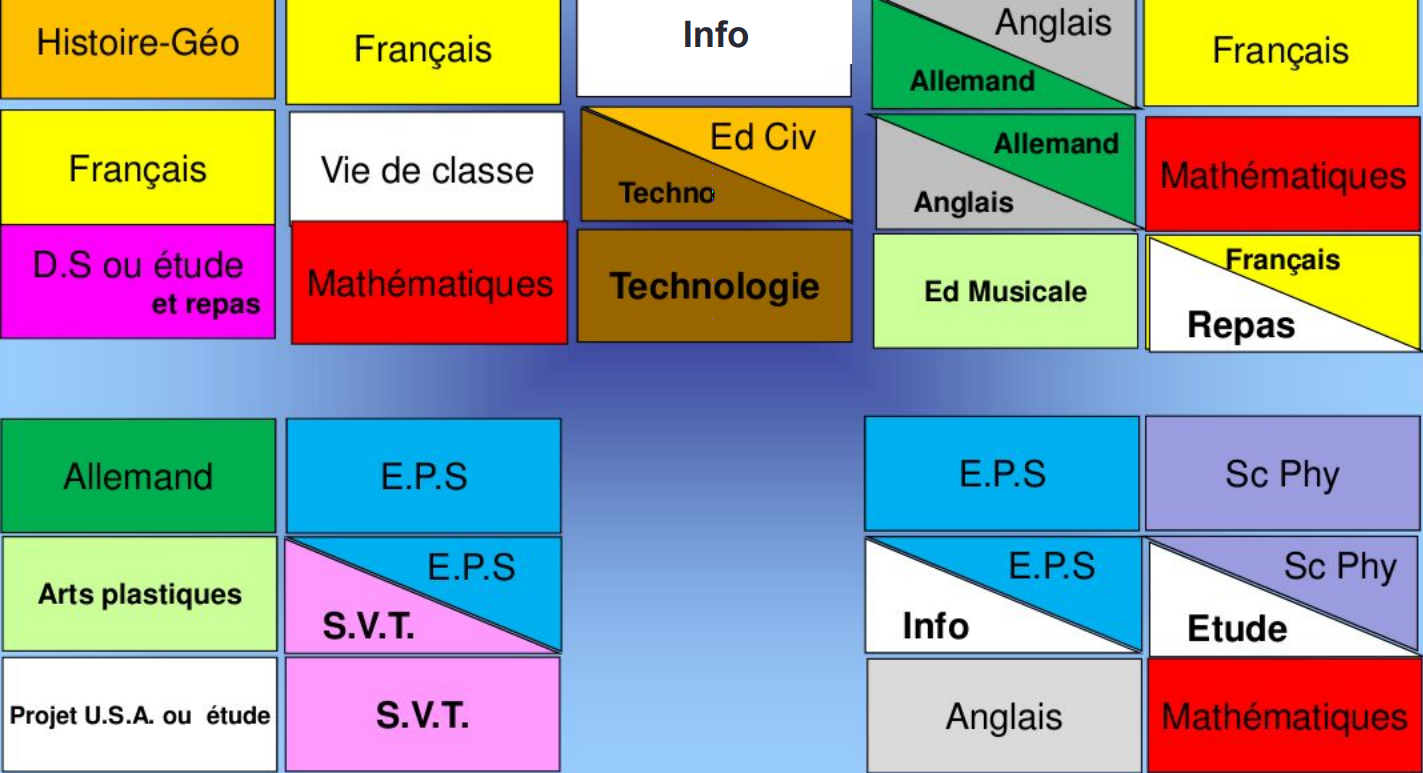
\includegraphics[width=17cm]{img/edt}\\

Il faudrait éviter au maximum les lundis et jeudis car j'ai les \textsc{NSI1} en demi-classe et cela déséquilibrerait mon planning de cours.\\
Je propose donc de caler les 3 jours sur un mardi, un mercredi et un vendredi, le tout sur la même semaine.\\
Le mardi et jeudi, on pourrait envisager de laisser les \textsc{NSI2} travailler en autonomie sur un projet.\\

Il ne faut pas tarder mais pas non plus se précipiter : pour composer les douze sujets nécessaires, il nous faut encore voir deux chapitres de mathématiques qui en font l'objet et l'actuel dispositif sanitaire n'arrange rien.

Je vous propose donc de vous contacter à nouveau dès que je pourrai estimer une semaine de passage.\\


Cordialement,
M. Leleu


\end{document}